\chapter{Thread handling}

Sometimes it is desirable to do calculations in a thread separate from an
applications main thread. Thread handling in HAPI is needed because haptics
rendering should be done at (at least) 1000 Hz which is considerably higher
than main loop threads of most applications. A typical application with haptics
added through HAPI would have thread communication like in figure \ref{threads}.
The purpose of the haptics thread is to calculate forces from all force effects
and geometries that are rendered on a haptics device (figure
\ref{haptics thread}).

\begin{figure} 
  \centering 
  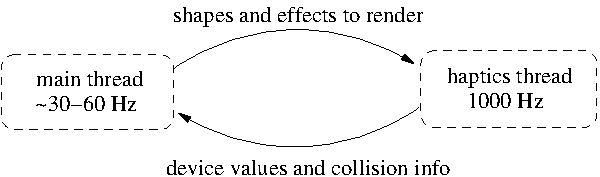
\includegraphics{images/threads.pdf}
  \caption{Thread communication}
  \label{threads} 
\end{figure}

\begin{figure} 
  \centering 
  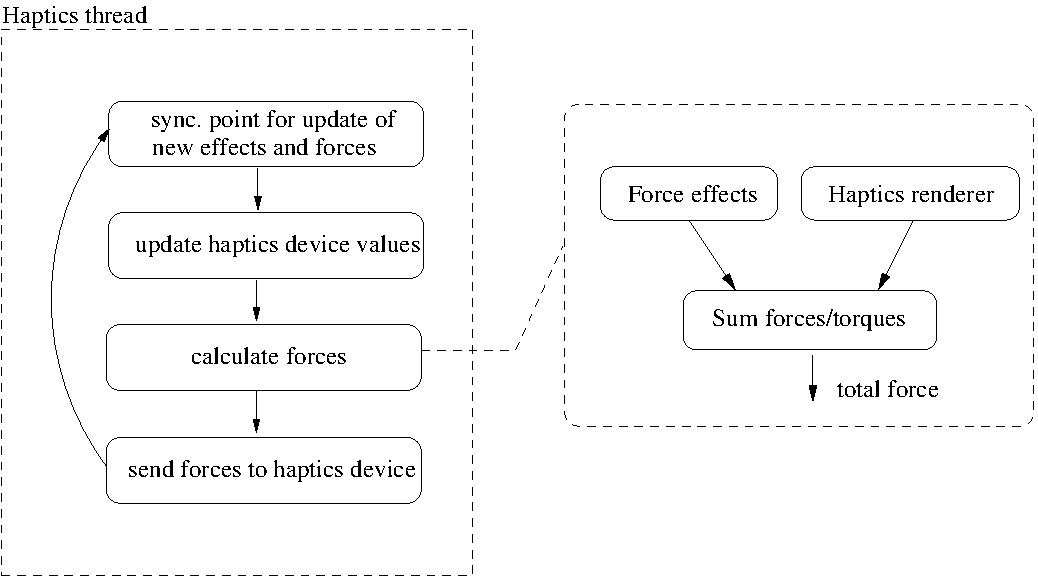
\includegraphics{images/hapticsthread.pdf}
  \caption{The flow of execution in the haptics thread.}
  \label{haptics thread} 
\end{figure}

\section{Thread handling classes}
All classes and everything needed to do proper thread handling in HAPI can be
found in the H3DUtil library. The most commonly used
classes for thread handling are:

\begin{itemize}
\item MutexLock - Used to lock/unlock access to data.
\item ConditionLock - A MutexLock with extra features.
\item SimpleThread - The simplest thread possible. Runs one function in a
separate thread.
\item PeriodicThread - Thread has a main loop and it is possible to add and
remove callbacks.
\end{itemize}

See doxygen documentation for Threads.h and Threads.cpp (in H3DUtil) for more
information and classes.

\section{Setting up a simple thread}
\label{secSimpleThread}
Setting up a thread using the SimpleThread class is very easy.
The arguments to SimpleThread are what function to run in a
separate thread and arguments to that function if there are any. If the
function depends on more than one argument these should be collected in a
custom made struct and a pointer to an instance of the struct should be sent
as argument.

A simple example of setting up a thread could be to print "SimpleThread"
over and over again to the console in a separate thread while the main thread
prints "Press ENTER to exit" once to the same console. The main thread will
wait for input from the user and when ENTER is pressed the program will exit.

\input{examples/SimpleThreadPrint_cpp.tex}

\section{Thread safety}
When adding new features which requires data to
be accessed by more than one thread care must be taken so that only one thread
at a time tries to access critical data. In HAPI this can be done in two ways.
One approach is to use callbacks, the other one is to use MutexLocks to lock
access for all other threads except the one that is currently modifying or
reading data. These approaches are not mutually exclusive. It is possible to
mix callbacks and locks.

\subsection{Using locks}
The concept of locks is easy to understand and use. The two most important
functions which exists in both the MutexLock class and ConditionLock class are:

\begin{itemize}
\item lock() - Used to lock access to data.
\item unlock() - Used to release the lock.
\end{itemize}

These two functions are used in pairs to protect code from being accessed by
more than one thread at a time. If a variable is used in two or more threads
there should be a lock/unlock pair around all code that use this variable. Similary, if a
function will be called from two or more threads all code in the function should
be enclosed by a lock/unlock pair. It is important to remember that calls to
the lock() function only prevent access to data surrounded by lock/unlock pairs
in those places where the same instance of MutexLock (or ConditionLock) is used
to lock. This means that in an application which contains "MutexLock A" and
"MutexLock B" calls to A.lock() will not prevent access to code after calls to
B.lock().

In the example in section \ref{secSimpleThread} one might want to change what
is printed to the console by the SimpleThread without setting up the thread
again. In the following example locks will be used in order to safely change
the content of the string variable used for printing since it is not possible
to set up callbacks for the class SimpleThread. Removing the locks from this
example will most likely crash the program when pressing ENTER.

\input{examples/SimpleThreadPrintLock_cpp.tex}

\subsection{Using callbacks}
Using callbacks is another way to handle thread safety. All threads that
inherit from the class PeriodicThreadBase must have the following functions
implemented.

\begin{itemize}
\item virtual void synchronousCallback( CallbackFunc func, void *data ) - Adds
  a callback function to be executed in this thread. The calling thread will
  wait until the callback function has returned before continuing.
\item virtual int asynchronousCallback( CallbackFunc func, void *data ) - Adds
  a callback function to be executed in this thread. The calling thread will
  continue executing after adding the callback and will not wait for the
  callback function to execute. Returns a handle to the callback that can be
  used to remove the callback.
\item virtual bool removeAsynchronousCallback( int callback\_handle ) - 
  Attempts to remove a callback. returns true if succeded. returns false if
  the callback does not exist. This function should be handled with care.
  Callbacks are removed if they return CALLBACK\_DONE or a call to this
  function is made.
\end{itemize}

The argument "func" in the above functions contains the callback function to
execute. The callback function has to be of the form
"CallbackCode myCallbackFunc( void *data )" where myCallbackFunc is the name of
the function. A callback function used with synchronousCallback shall
return the CallbackCode CALLBACK\_DONE. A callback functions used with
asynchronousCallback should return either CALLBACK\_DONE or CALLBACK\_CONTINUE.
As long as the return code is CALLBACK\_CONTINUE the callback will be called in
the next thread loop.

Here follows an example on how to create a thread and set up different
callbacks.

\input{examples/PeriodicThreadCallbacks_cpp.tex}

For thread safety reasons it does not matter if we add the function
printSynchronous as a synchronousCallback or asynchronousCallback. The program
will not crash. The only difference is that the calling thread will wait for
the callback to finish before continuing. However, if the main thread would
change the value of the variable "to\_print" without the use of callback a
crash may occur. It is more likely to happen for high update frequencies of the
PeriodicThread.

\section{Threads and haptics devices}
Haptics rendering have to be done for each device which means that each device
will have its own haptic thread. Most of the time it is enough to use the
functions in section \ref{ssHapticsRenderingFunctions} but sometimes one might
want to access the thread of the haptics device. This can be done through the
function "H3DUtil::PeriodicThreadBase *getThread()" defined in the
HAPIHapticsDevice class. The thread returned from this function can be used
to set up new callbacks.

By default the thread used is a HapticThread. Most of the time when adding a
new device to HAPI by subclassing HAPIHapticsDevice the default thread is
sufficient. If however the haptics device provides some way of adding callbacks
through calls to other functions a wrapper class should be implemented
to override the virtual functions of PeriodicThreadBase for adding and removing
callbacks. For example implementation of this see HLThread and PhantomHapticsDevice.